\chapter{La base de données comme réponse à des besoins : datavisualisations, enrichissements et possibilités offertes par ce projet}

Comme nous l'avons évoqué, \emph{Heurist}\index{Heurist} est utilisé pour sa capacité à satisfaire de nombreux besoins, auxquels notre travail a pour but de répondre. 

\section{Enrichissements de la base par des informations extérieures aux factures}

Si le besoin essentiel auquel doit répondre la base est, nous l'avons vu, de transcrire les factures, elle doit aussi prévoir la possibilité d'être complétée par des informations venues de sources extérieures.
L'utilité principale est de nous renseigner davantage sur ce que l'on recherche dans la base si les seules informations présentes dans les factures sont lacunaires. C'est pourquoi une partie des champs du \emph{Record type} \enquote{ligne de facture} sert à accueillir des données issues des catalogues en ligne de la BnF contenant les oeuvres de la collection Rondel, à savoir le catalogue général\index{Catalogue général de la BnF} ou BnF Archives et Manuscrits\index{Bnf Archives et manuscrits}. 

\begin{figure}[htbp]
    \centering
    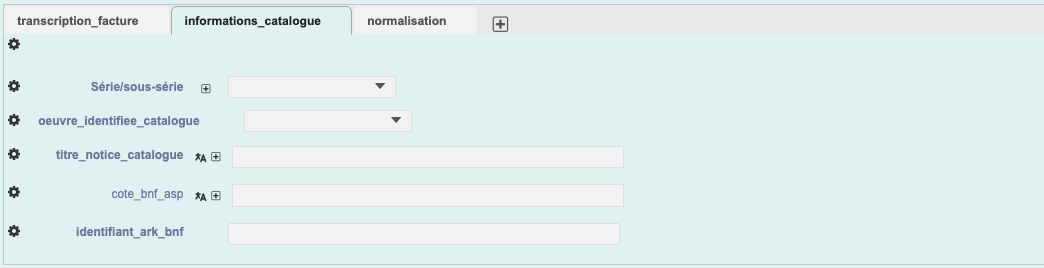
\includegraphics[width=12cm]{Images/informations catalogue_2.png}
    \caption{Section \enquote{Informations catalogue} dans le \emph{Record type} \enquote{ligne de facture}.}
    \label{fig:informations-catalogue}
\end{figure}

\newpage
Comme nous le montre l'image ci-dessus, \emph{Heurist}\index{Heurist} permet de diviser chaque \emph{Record type} en plusieurs sections, appelées \emph{Tabs}. Grâce à cela, nous avons pu distinguer clairement dans une \emph{Tab} appelée \enquote{transcription factures} les données issues des factures, et dans une autre nommée \enquote{informations catalogues} celles trouvées dans les catalogues de la BnF, car comme nous l'avons vu, il est essentiel dans la saisie de données d'indiquer l'origine des informations. Ces champs sont très importants dans notre travail, parce qu'ils permettent de retrouver, dans les catalogues de la BnF, les oeuvres indiquées dans les factures, et de faire un lien entre les deux. En effet, un champ est prévu pour indiquer la cote de l'ouvrage au sein de la collection, lorsque celle-ci est clairement identifiée. Un autre champ permet de sélectionner la série et/ou la sous-série à laquelle l'oeuvre appartient à l'aide d'un vocabulaire renseignant le nom de cet ensemble, et l'intervalle de cote associé, pour pouvoir l'associer à l'oeuvre avec certitude. 

\begin{figure}[htbp]
    \centering
    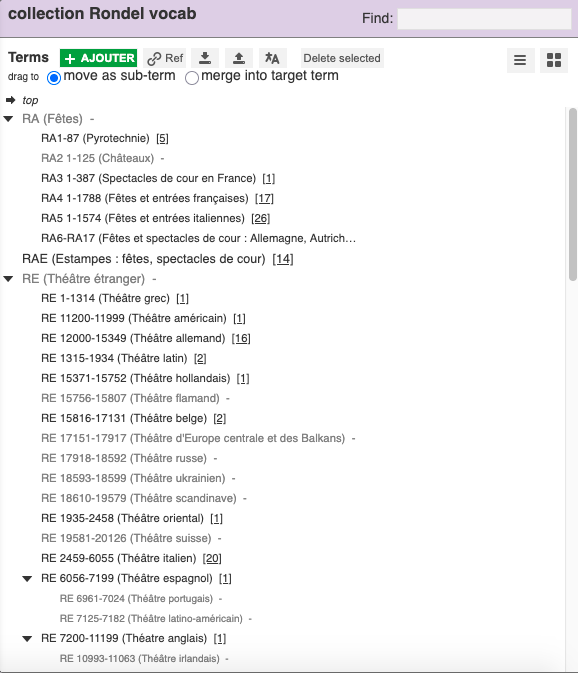
\includegraphics[width=12cm]{Images/collec_Rondel_vocab.png}
    \caption{Vocabulaire contrôlé qui recense les différentes séries et sous-séries de la collection Rondel, et leurs intervalles de cotes respectifs.}
    \label{fig:vocabulaire-collection-rondel}
\end{figure}
\newpage


Il est donc parfois possible, en complétant avec des informations venant des catalogues, de retrouver avec précision la provenance d'un exemplaire de la collection Rondel.

Ce principe de champs spécialement prévus pour les ajouts d'informations extérieures, à bien séparer dans des sections distinctes de ce qui provient des factures, a également été utilisé dans la table \enquote{personne} de notre base, cette fois pour donner la possibilité d'approfondir la recherche sur des personnes. Cela entend répondre au besoin, identifié lors du travail préparatoire à la modélisation, de s'intéresser plutôt aux libraires. Ces champs, non obligatoires, n'ont pas vocation à être remplis systématiquement lorsqu'on saisit une personne dans la base, mais anticipent plutôt des potentiels usages prosopographiques sur des libraires. Ainsi, nous avons ajouté dans la table \enquote{personne} une section \enquote{enrichissements}, notamment constituée des dates de naissance et de mort des personnes, et des champs voués à l'ajout d'informations biographiques et à l'indication des sources utilisées.
Afin d'expérimenter ces champs, mais également d'autres possibilités offertes par la base, nous avons décidé de sortir de l'échantillon que nous utilisions au départ, et de mener nous-mêmes des recherches approfondies sur un ou des libraires en particulier. Cela nous a amené à nous intéresser à la famille Saffroy, une grande famille de libraires ayant exercé son activité à Paris et au Pré-Saint-Gervais entre 1880 et 2020\footcite{magazine_famille_2021}. Nous avons découvert cette famille en examinant les titres des dossiers qui composent notre corpus, et en remarquant qu'Auguste Rondel a été client de plusieurs membres de cette famille\footnote{Les dossiers concernant la famille Saffroy sont dans le catalogue BnF Archives et Manuscrits sous les cotes RCOL-1(382) à (386).}. Notre recherche s'est donc focalisée sur cette famille, et nous avons renseigné dans la base tous ses membres qui apparaissent dans les factures, leurs proches, et les liens qui les unissent. 

En somme, si cette base garde pour fonction principale d'accueillir un maximum d'informations des factures, elle a pour visée secondaire de permettre l'ajout d'informations extérieures, pour la compléter et approfondir les recherches. Cependant, il doit être possible d'identifier clairement la source de toutes les données présentes dans la base. 

\newpage 
\section{Interopérabilité, liens avec d'autres logiciels et réutilisation des données}

Cette base de données entend exploiter les possibilités d'\emph{Heurist} pour répondre, dans la mesure du possible, à des enjeux essentiels dans les projets de recherche : la conformité aux objectifs de la science ouverte et le respect des principes FAIR (\emph{Findable}, \emph{Accessible}, \emph{Interoperable}, \emph{Reusable}). 

Pour ce faire, l'enrichissement de la base avec des informations extérieures peut servir à y intégrer  des formats interopérables, en liant les données à des concepts universels et identifiés de manière unique sur le web. L'enjeu est de se rapprocher de l'ambition portée par le web de données. Théorisé dès 1998 sur la feuille de route pour le web sémantique de Tim Berners-Lee par l'expression \emph{Web of data}, le web de données est une vision du web proposant une interopérabilité fondée sur la création d'un espace global d'information où toutes les données sont liées entre elles, et sont compréhensibles par les machines\footcite{bermes_2_2013}. C'est pourquoi l'un des champs de la section \enquote{informations catalogue}, appelé \enquote{identifiant ark bnf}, est prévu pour accueillir l'identifiant ARK associé à chaque oeuvre identifiée dans le catalogue. De même, la section \enquote{enrichissements} de la table \emph{personne}, présentée dans la partie précédente, contient un champ appelé \enquote{notice autorité} prévue pour indiquer, s'il existe, l'identifiant ARK de l'autorité BnF de la personne que l'on saisit. 
L'\emph{Archival Resource Key} est un système fournissant des URL stables pour les ressources numériques, utilisé dans les institutions patrimoniales, et notamment dans les bibliothèques\footcite[p. 34]{hervieu_2024}. L'ARK est un identifiant pérenne faisant partie des données d'autorité qui contrôlent la description des ressources de la BnF, c'est pourquoi il est nécessaire de pouvoir s'y référer depuis notre base de données\footcite{noauthor_donnees_nodate}. 

Dans ce même but, tous les noms de lieux associés à des librairies sont indexés dans des formats interopérables, afin d'être rattachés à des standards universels, à des référentiels exposés sur le web\footcite[Voir \enquote{Présentation de Heurist}]{paillusson_introduction_2022}. Cette possibilité est offerte par les vocabulaires contrôlés d'\emph{Heurist}\index{Heurist}, dont les termes peuvent être associés à une URI cliquable. Ainsi, les noms de villes et de pays indexés dans notre base sont tous reliés à des identifiants \emph{GeoNames}\index{GeoNames}, une base de données géographique mondiale recouvrant plus d'onze millions de lieux\footcite{noauthor_geonames_nodate}. 

\begin{figure}[htbp]
    \centering
    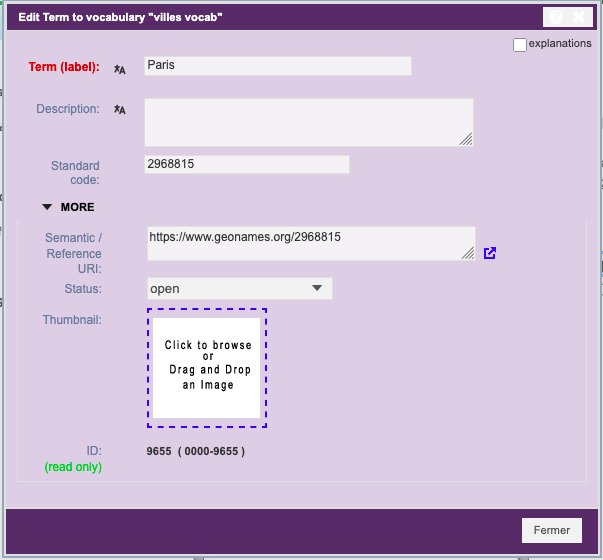
\includegraphics[width=12cm]{Images/lieux_web_semantique.png}
    \caption{ville de Paris identifiée dans la base et liée à \emph{GeoNames} conformément aux principes de mise à disposition des données dans le cadre du web sémantique (ces identifiants sont exprimés par des URI, et formulés grâce au protocole HTTP, pour qu'on puisse y accéder).}
    \label{fig:paris-geonames}
\end{figure}



\newpage


La compatibilité avec d'autres logiciels peut également servir à enrichir rapidement et automatiquement une base par l'import de données du web. Ce besoin est notamment assuré par la fonction de synchronisation entre \emph{Heurist}\index{Heurist} et \emph{Zotero}\index{Zotero}, un logiciel libre, gratuit et simple d'utilisation permettant de collecter, d'organiser, d'annoter, de citer et de partager des ressources bibliographiques\footcite{noauthor_zotero_nodate}. 
La synchronisation possible entre les deux logiciels permet donc d'importer, dans une base \emph{Heurist}\index{Heurist}, des notices bibliographiques complètes et générées avec \emph{Zotero}\index{Zotero}. Cette opération est possible grâce à une clé API, et à un identifiant appelé \emph{User ID}, qu'il nécessaire de récupérer sur le site zotero.org. Ces identifiants sont à renseigner ensuite dans \emph{Heurist}\index{Heurist}, en suivant des étapes énumérées dans le guide sur les usages de la base\footnote{Voir à la page 16 de l'annexe C - I. \enquote{ \nameref{documentation}}}. Dès lors, la synchronisation entre les deux logiciels se fait immédiatement, et peut être mise à jour à tout moment en appuyant simplement à nouveau sur le bouton dédié. Les données issues de \emph{Zotero}\index{Zotero} apparaissent dans des enregistrements spécifiques, chacun étant consacré à une ressource. Cette possibilité sert à enrichir rapidement une base de données avec tous types d'informations issues du web, ou de sourcer plus facilement les informations de la base. Il s'agit aussi d'une preuve supplémentaire de la pertinence d'\emph{Heurist} dans les projets en sciences humaines, car le logiciel est compatible avec d'autres outils courammment utilisés dans la recherche. 
Cependant, cette synchronisation présente des limites. En effet, il n'est pas possible de contrôler l'endroit où vont les données de \emph{Zotero}, en prévoyant des champs adéquats dans la base. Les données ne sont pas visibles directement au sein des \emph{Record types}, mais sont classés par types de ressources (\emph{Book}, \emph{Web Bookmark}, ...). Pour les faire apparaître dans la base, nous avons donc créé un champ au sein de la table \enquote{personne} faisant le lien entre une personne et une ressource Zotero\index{Zotero}. Cet exemple montre une autre façon d'associer, à une base Heurist\index{Heurist}, des données du web.  

En plus de pouvoir être liées à des standards universels et d'être intégrées au web, les données \emph{Heurist}\index{Heurist} sont exportables dans des formats ouverts, et réutilisables dans de nombreux autres logiciels. Elles peuvent par exemple être exportées en CSV, XML ou JSON, mais également être importées dans \emph{Heurist}\index{Heurist} dans les mêmes formats\footcite[Voir \enquote{Présentation de Heurist}]{paillusson_introduction_2022}. Cette réutilisation possible des données a également répondu aux besoins de notre projet, car certains traitements que nous souhaitions réaliser étaient impossibles avec \emph{Heurist}\index{Heurist}. Le logiciel ne permet pas de réaliser des calculs précis. Or, la base de données a aussi parmi ses objectifs de nous renseigner sur les dépenses effectuées par Auguste Rondel dans sa collection. Cela explique pourquoi plusieurs champs du \emph{Record type} \enquote{facture} sont consacrés aux prix totaux, aux frais et aux devises renseignés dans les factures. Nous avons donc exporté cette table en format CSV afin de pouvoir réaliser les calculs dont nous avions besoin grâce à des formules Excel\index{Excel}. Les formules étaient très simples : il s'agissait de multiplications, dans le but de convertir en francs tous les prix totaux et les frais payés par Auguste Rondel. Les conversions ont été effectuées depuis toutes les monnaies que nous avions dans l'échantillon (franc suisse, lire, livre, mark et Reischmark), et grâce à un taux de change déterminé avec l'outil currency converter de Historical statistics\footcite{noauthor_historical_nodate}. Une fois ces calculs faits, nous avons importé le fichier CSV avec tous les prix normalisés en franc dans la base. Tout ce procédé, dont il ne faut pas oublier les biais et le caractère expérimental, est lui aussi détaillé dans la documentation sur les usages ultérieurs de la base\footnote{Voir \enquote{ \nameref{documentation}}}. Il convient surtout de retenir de cet exemple que les données \emph{Heurist}\index{Heurist} peuvent facilement être exportées et importées dans des formats ouverts, ce qui permet de les réutiliser dans d'autres cadres, au-delà du logiciel lui-même. 

\section{Requêtes et visualisations possibles à partir de la base}

Après nous être intéressés à l'intégration de données extérieures dans la base, et aux besoins auxquels nous tentons de répondre en matière de science ouverte, il convient de nous pencher sur les différents moyens d'interroger les données et les visualiser. 

\vspace{1.5cm}

L'un des intérêts d'une base de données relationnelles est de pouvoir interroger ses données. Cela fait partie des raisons de l'utilisation d'une base de données dans notre projet, car la finalité de collecter autant de données issues des factures est de pouvoir les interroger, les manipuler, se focaliser sur certains aspects, dans le but d'en extraire des statistiques, de les visualiser ou encore de les publier. Dans la plupart des SGBDR (Système de gestion de bases de données relationnelles), l'interrogation des tables d'une base se fait, comme nous l'avons vu dans le chapitre 3, grâce au langage SQL. Cependant, comme l'utilisation de notre base se veut être accessible à un public large, il est nécessaire de pouvoir interroger la base sans avoir à coder. Pour cela, \emph{Heurist} prévoit plusieurs manières d'interroger un ou plusieurs \enquote{Record types}. 
Tout d'abord, chaque table peut être interrogée séparément par des filtres. Il suffit d'utiliser le mode \emph{Explore}, et de créer un filtre grâce à l'icône représentant un entonnoir. Le filtre permet de ne sélectionner, au sein d'une table, que les enregistrements répondant à certains critères. Il est également possible d'enregistrer les filtres créés, et de les conserver ensemble grâce à la rubrique \emph{Saved filters}. Une fois les filtres enregistrés, on peut accéder à la requête produite par \emph{Heurist} à partir de ce qu'on a sélectionné. 
Ces filtres sont l'équivalent des requêtes SELECT en SQL, qui permettent d'extraire d'une base de données les données répondant à des questions que l'on peut se poser\footcite[p. 203]{Hainaut_2015}. 
Cette fonctionnalité d'\emph{Heurist} est très adaptée à notre projet de recherche, car celui-ci entend pouvoir se focaliser sur des thématiques particulières, comme par exemple une typologie de documents, ou un libraire en particulier. Les images ci-dessous montre les requêtes issues de plusieurs filtres réalisés dans le cadre de notre travail. 

\begin{figure}[htbp]
    \centering
    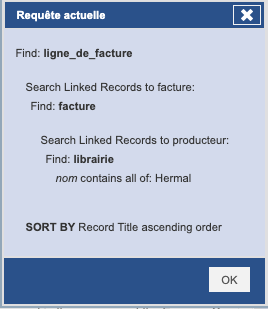
\includegraphics[width=5cm]{Images/requete_Hermal.png}
    \caption{Cette requête sélectionne, dans la table \enquote{ligne de facture}, toutes les lignes liées à un enregistrement \enquote{facture}, eux-mêmes liés à un  enregistrement \enquote{librairie} qui contient le mot \enquote{Hermal}, et trie les titres par ordre alphabétique. En somme, elle ne sélectionne que les documents achetés par Rondel à la librairie Hermal.}
    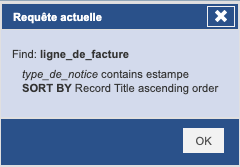
\includegraphics[width=5cm]{Images/requete_estampes.png}
    \caption{Cette requête sélectionne toutes les lignes de facture dont le champ \enquote{type de notice} contient le terme \enquote{estampe}, et trie les titres par ordre alphabétique. Elle ne sélectionne donc que les estampes.}
    \label{fig:requetes-heurist}
\end{figure}

Cependant, les possibilités de requêtes dans \emph{Heurist} sont très limitées par rapport à celles du langage SQL. Par exemple, les filtres du logiciel ne permettent pas d'interroger plusieurs tables en une seule requête, comme le font les jointures (\emph{join}) en SQL\footcite[p. 228]{Hainaut_2015}. 

Pour faciliter l'interrogation de la base, nous avons surtout opté pour la deuxième possibilité offerte par \emph{Heurist}\index{Heurist}, à savoir les \emph{Faceted search}, ou \enquote{filtres à facettes}. Il s'agit d'un mode de navigation structurée permettant de filtrer une recherche dans la base à l'aide de nombreux critères, correspondant aux différents champs de la base et pouvant prendre la forme de recherche plein texte, de listes de sélection ou encore de cases à cocher\footcite[\enquote{Création d’un filtre de recherche à facettes}]{paillusson_introduction_2022}. Sorte de recherche avancée au sein d'une base Heurist\index{Heurist}, les facettes permettent de se concentrer plus précisément sur certaines propriétés d'une ou plusieurs tables\footcite[Filter-Edit-Analyse-Publish]{noauthor_faceted_nodate}. 

\begin{figure}[htbp]
    \centering
    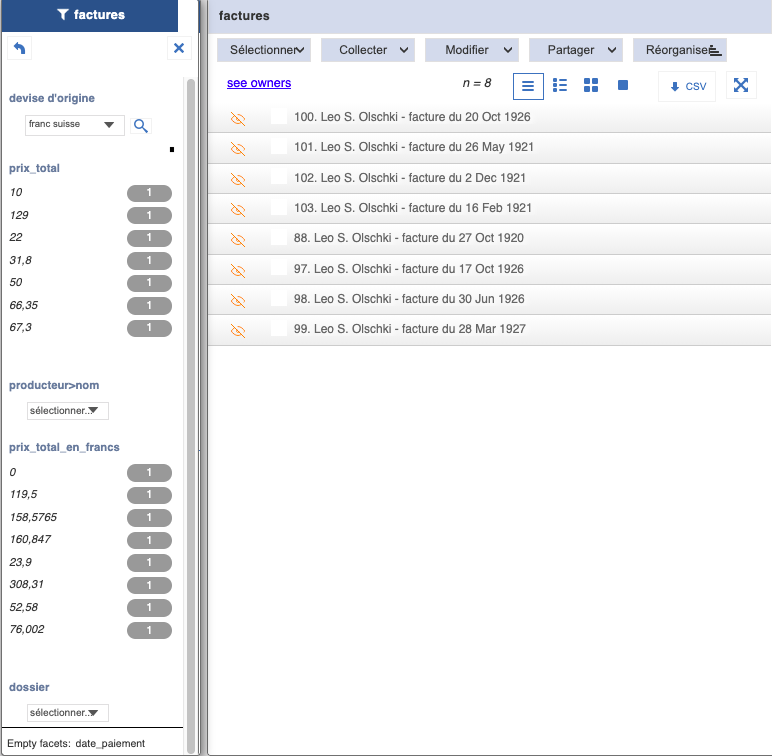
\includegraphics[width=15cm]{Images/facet_factures.png}
    \caption{Recherche à facettes sur la table \enquote{facture}, qui n'interroge ici que les factures payées en francs suisses.}
    \label{fig:facettes-factures}
\end{figure}

Dans ce projet, les facettes sont privilégiées aux filtres, car elles ressemblent davantage aux formes de recherches avancées que l'on peut trouver habituellement dans les catalogues de bibliothèques ou sur d'autres sites internet. Elles paraissent donc plus simples à prendre en main par un public large. 

Comme nous l'avons vu, interroger cette base de données nous permet de répondre à certains enjeux du projet de recherche en cours, en se focalisant sur certains de ses aspects en particulier. L'interrogation des données doit être comprise conjointement à leur visualisation, car les données sont souvent interrogées dans le but d'être visualisées. 

\vspace{1.5cm}

La datavisualisation se définit par sa capacité à présenter rapidement les données et à les rendre lisibles\footcite[p. 11]{lagnel_2021}. Elle est une attente majeure de ce projet, car cela matérialise ce que nous disent les factures Rondel sur tous les sujets qu'elles permettent d'étudier. Il s'agit de l'un des intérêts d'\emph{Heurist}\index{Heurist} qui, nous l'avons évoqué, est pensé pour répondre aux problématiques des SHS, intégrant donc nativement diverses possibilités de visualisation\footcite[\enquote{Présentation de Heurist}]{paillusson_introduction_2022}. Notre projet de recherche a donc produit différents types de visualisations en lien avec les questions qu'il entend traiter. 

Conformément aux objectifs du projet, les factures Rondel peuvent largement être exploitées pour étudier les réseaux de libraires. Le logiciel est très utile par sa capacité à créer des graphes, de manière à représenter les relations de la base sous forme de réseau. La visualisation du réseau standard est constitué de noeuds (points), et d'arêtes (ligne qui les relie)\footcite[p. 189]{Drucker_2020}. C'est le principe de la fonction \emph{Network}, au sein du mode \emph{Explore} du logiciel, qui affiche sous la forme d'un réseau toutes les relations enregistrées dans une table. Dans le chapitre 5, nous avons vu que l'exploitation des factures a permis de saisir et de caractériser de manière précise de nombreuses relations entre des personnes ou des libraires indexées dans la base\footnote{Voir p.\pageref{conception base}}. Toutes ces relations sont donc modélisables sous forme de graphes, et visibles directement dans \emph{Heurist}\index{Heurist}. Les réseaux créés à partir de la base sont visibles et expliqués dans les annexes\footnote{Voir dans l'annexe D, \enquote{ \nameref{reseaux heurist}}.}. 
La visualisation de réseaux est, nous l'avons vu, disponible nativement avec \emph{Heurist}. Cependant, il est également possible, si l'on souhaite approfondir cette question, d'exporter les données concernées en un fichier de graphe au format .gexf, et de visualiser les réseaux grâce au logiciel gephi\index{Gephi}. Ce logiciel permet d'explorer, de manipuler et de comprendre des réseaux complexes\footcite{noauthor_gephi_nodate}, et a été expérimenté dans le cadre de ce travail sur l'ensemble des relations de la table \enquote{personne}\footnote{Voir l'annexe \enquote{\nameref{reseau gephi}}.}.


Les données issues des factures permettent aussi d'étudier spatialement les librairies où Rondel s'est fourni. En effet, il est possible d'utiliser \emph{OpenStreetMap}\index{OpenStreetMap} au sein même de la base \emph{Heurist}\index{Heurist}, afin de produire des visualisations cartographiques. Le principe est simple : il suffit de créer un champ de type \emph{geospatial} afin d'y saisir des noms de lieux ou d'adresses, qui seront ensuite géoréférencés. La visualisation d'une carte montrant tous les lieux géoréférencés est alors permise par une autre fonction du mode \emph{Explore}, appelée \emph{Map}. Dans le cadre du projet de recherche sur les factures Rondel, cela permet, grâce à la création d'un champ \enquote{coordonnées géographiques} au sein de la table \enquote{lieu}, de produire une carte de tous les libraires où Auguste Rondel s'est fourni\footnote{Voir l'annexe \enquote{\nameref{cartes heurist}}.}. Dans ce cas précis, il peut être particulièrement intéressant de produire une carte à partir d'une requête, car l'un des enjeux du projet est, on le rappelle, de pouvoir se concentrer sur une thématique en particulier, comme une aire géographique. Ainsi, il est tout à fait possible, par un filtre, de n'afficher sur une carte que les librairies parisiennes par exemple. 

Comme les réseaux, les données cartographiques indexées peuvent être visualisées à l'intérieur même de la base \emph{Heurist}\index{Heurist}, mais peuvent aussi être exportées dans des formats spécifiques, pour exploiter les possibilités de logiciels plus spécialisés. Il est possible d'exporter ces données au format KML (\emph{Keyhole Markup Language}), format de données XML utilisé pour afficher des informations dans un contexte géographique\footcite{francois_kml_2017}. Nous avons utilisé l'autre possibilité, à savoir l'export en GeoJSON, format d'encodage de données géospatiales basé sur \emph{Javascript Object Notation} (JSON). Ce dernier nous a servi à exporter nos données géospatiales pour les réutiliser dans le logiciel QGIS\index{QGIS}, logiciel libre de système d'information géographique (SIG) permettant notamment de créer et d'annoter des cartes. Ce logiciel a surtout été utilisé pour tester l'export de données GeoJSON depuis \emph{Heurist}. Ce logiciel a donné la possibilité de récupérer toutes les données géospatiales de la table \enquote{lieu}, de les placer sur un fonds de carte \emph{OpenStreetMap}\index{OpenStreetMap}, et d'en créer un fichier PNG avec une légende\footnote{Voir l'annexe \enquote{\nameref{carte qgis}}.}. Ces fonctionnalités minimales de QGIS\index{QGIS} ont été utilisées à titre d'exemple, mais le logiciel offre de nombreuses autres possibilités à partir de données géospatiales. 


Ces pratiques cartographiques ont ouvert la voie à d'autres expérimentations, reposant également sur le principe de géoréférencement. Toujours dans le but de cartographier les librairies, y compris en se concentrant sur une aire géographique précise, nous avons expérimenté l'outil GALLIGEO\index{Galligeo}, qui permet, grâce au géoréférencement par points de contrôle, de produire une visualisation spatiale sur des cartes anciennes disponibles sur Gallica\index{Gallica}, bibliothèque numérique de la BnF\footcite[p. 27]{hervieu_2024}. Tout comme l'outil cartographique d'\emph{Heurist}, GALLIGEO\index{Galligeo} utilise une carte \emph{OpenStreetMap}\index{OpenStreetMap}, sur laquelle on peut renseigner les adresses une fois que la carte est géoréférencée. L'usage de cet outil pour exploiter les factures Rondel est complètement extérieure à toute utilisation d'\emph{Heurist}, mais peut servir à certaines études de cas. Par exemple, nous avons utilisé GALLIGEO\index{Galligeo} pour géoréférencer toutes les librairies marseillaises où Rondel s'est fourni, sur un fonds de carte datant de 1931\footnote{Voir l'annexe \enquote{\nameref{carte galligeo}}.}. Tout comme dans la base \emph{Heurist}\index{Heurist}, cette étude a permis de visualiser spatialement les librairies, mais en se rapprochant davantage des réalités de l'époque. 

\vspace{1.5cm}
Il faut noter que d'autres formes de datavisualisation sont possibles, mais qu'elles ont été experimentées de manière plus secondaire pour exploiter les données des factures Rondel. L'outil \emph{Crosstabs}, ou \emph{cross-tabulation}\footcite{noauthor_crosstabs_nodate}, permet de faire des calculs sur les données d'un \emph{Record type}, et d'en représenter les résultats sous forme de tableau, ou de graphique sectoriel, aussi appelé \emph{Pie chart} ou plus familièrement \enquote{camembert}. 
Cette fonction est accessible dans le mode \emph{Explore}, et pour l'utiliser, il suffit de sélectionner le \emph{Record type} et les champs concernés. 
Il serait très intéressant d'utiliser les \emph{Crosstabs} ultérieurement avec cette base, car cet outil permettrait de faire des statistiques sur la collection Auguste Rondel, ou sur la base de données en elle-même. Cependant, la base ne contient pas assez de données à ce stade pour que des statistiques soient représentatives. Nous avons malgré tout expérimenté cette possibilité à plusieurs reprises. En voici un exemple : 


\begin{figure}[htbp]
    \centering
    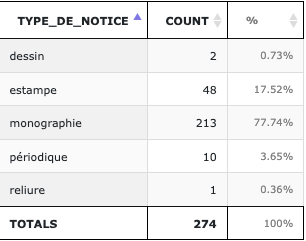
\includegraphics[width=0.5\textwidth]{Images/tableau_typo_documents.png}
    \caption{\emph{Crosstab} faisant une typologie des documents indexés dans la base.}
    \label{fig:crosstab-typologie}
\end{figure}

\begin{figure}[htbp]
    \centering
    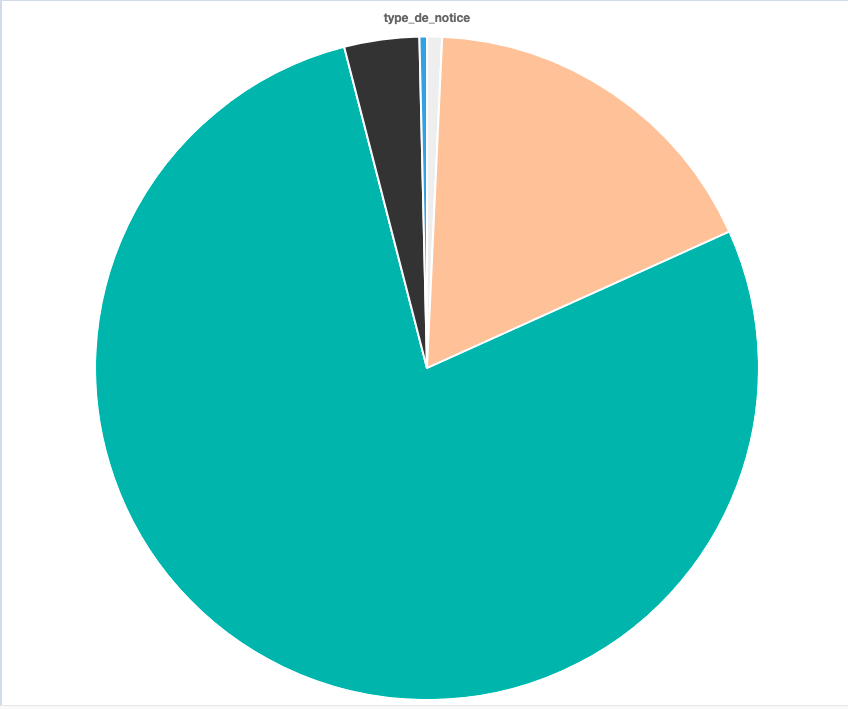
\includegraphics[width=0.5\textwidth]{Images/graphique_typo_documents.png}
    \caption{Mêmes données que sur l'image précédentes, cette fois affichées sous la forme d'un graphique sectoriel.}
    \label{fig:graphique-typologie}
\end{figure}

\clearpage 
Dans le cas présent, ce graphique contient peu de catégories, c'est pourquoi il est lisible. Toutefois, ce type de visualisation est déconseillé au-delà de six catégories car les parts sont trop petites, donc l'oeil n'arrive plus à différencier les proportions\footcite[p. 83]{lagnel_2021}. Ainsi, même si elle est simple d'utilisation et intégrée à \emph{Heurist}\index{Heurist}, cette datavisualisation n'est pas toujours intéressante et est à limiter à certains cas. Cette forme de graphique est la seule visualisation possible dans \emph{Heurist}\index{Heurist} à partir des \emph{Crosstabs}. Si l'on souhaite d'autres représentations graphiques à partir des données Heurist, il reste possible d'exporter les données et de les réutiliser dans un logiciel adapté, comme \emph{Tableau}\index{Tableau}, logiciel de référence en matière de datavisualisation. 

Toutes ces possibilités d'interrogation et de visualisation de la base servent donc à exploiter nos données de recherche. Elles peuvent également avoir pour but de préparer les données afin de les rendre accessibles à un public large\footcite[\enquote{Mettre en ligne les données gérées dans Heurist}]{paillusson_introduction_2022}. 

\section{Favoriser l'accessibilité des données et mettre en valeur le travail : un site internet conçu à partir de la base}

La base doit pouvoir être publiée et documentée. Cet impératif répond au besoin de valoriser ce projet de recherche en cours, mais aussi de garantir l'accessibilité des données, conformément, là encore, au principes de la science ouverte. C'est pourquoi nous avons utilisé la possibilité, intégrée à \emph{Heurist}\index{Heurist}, de créer un site web à partir de la base de données\footnote{Le lien vers le site web est disponible dans les annexes, dans la section \enquote{\ref{website}}.}. En effet, le mode \emph{Publish} du logiciel permet de publier les données sur le web sous la forme d'un CMS. Cet acronyme signifie \emph{Content Management System}, et désigne un programme informatique permettant de gérer l'apparence et le contenu d'un site web de manière centralisée\footcite{noauthor_content_nodate}. 

Contrairement à des sites web HTML plus classiques, les sites générés à partir d'\emph{Heurist} ne sont pas développés avec un code HTML complet\footcite[Le langage HTML (\emph{Hypertext Markup Language}), est un langage de programmation déclarative, de description de l'information]{margaux_faure_2025}, assorti d'une feuille de style CSS\footcite[Le langage CSS (\emph{Cascading Style Sheets}), permet de travailler l'apparence d'un site web en lui appliquant des règles de style]{margaux_faure_2025}. 
Une fois généré par le bouton \emph{Create} du mode \emph{Publish} et ouvert en mode \enquote{édition}, le site peut être agencé à l'aide de la fonction \emph{Website editor}. Les pages du site sont choisies parmi des formes pré-conçues prévues par \emph{Heurist}\index{Heurist}. Son contenu textuel est géré par des bouts de code HTML à placer dans des formulaires de saisie répartis à différents endroits de l'éditeur du site. L'esthétique du site (polices d'écriture, couleurs, ...) est définie par des bouts de code en CSS, également à saisir dans des formulaires. Le site créé dans le cadre de notre projet s'est inspiré de l'agencement des pages et du texte des sites générés à partir des autres bases \emph{Heurist} de la BnF. Nous avons aussi repris les bouts de code CSS de ces autres sites pour les injecter dans le nôtre, ce qui a nécessité quelques modifications pour les ajuster au contenu de notre site. Ce choix a été fait dans un souci de cohérence avec les pratiques de l'institution, afin d'inscrire notre base dans la continuité des projets similaires menés à la BnF. L'intérêt principal du site web, à savoir l'accès aux données de la base, réside dans les filtres et \emph{facets} évoqués dans la partie précédente. Ces modes d'interrogation de la base sont réutilisables dans le site web, ce qui donne un accès direct aux données par des recherches avancées et des visualisations. Chaque table de la base sur les factures Rondel est donc interrogeable dans le site sur une page dédiée. La page \enquote{lieu} donne accès à la carte des lieux indexés dans la base, et la page \enquote{personne} aux réseaux de libraires. Les pages \enquote{facture} et \enquote{ligne de facture} permettent, quant à elles, d'interroger respectivement les deux tables par de nombreux filtres de recherche. Il faut noter que le site web permet de retrouver n'importe quelle donnée de la base grâce à des barres de recherche plein texte réparties sur les différentes pages du site. 

Ce site web répond donc au besoin de publicité et d'accessibilité des données. Cependant, il comporte certaines limites et incertitudes, spécifiques aux sites web \emph{Heurist}\index{Heurist} ou plus générales. Si un site web CMS correspond aux objectifs d'Heurist, à savoir permettre une utilisation minimale de programmation pour en élargir l'accès, cela n'est valable que pour le développement d'un site web minimaliste. Si l'on souhaite personnaliser l'esthétique et la forme ou l'adapter à une forme standard, comme nous l'avons fait dans le cadre de ce projet, l'édition requiert certaines compétences en développement web. De plus, développer un site web par petits bouts de code éparpillés est très déroutant, et la documentation n'est pas suffisante pour en comprendre précisément le fonctionnement. 

\vspace{1.5cm}
Enfin, la création de ce site web a suscité quelques questions, pour l'instant restées en suspens et au stade expérimental. Nous nous sommes interrogés sur un potentiel besoin d'avoir des formes normalisées des principales informations sur les oeuvres. Cette réflexion est partie du constat que des informations importantes peuvent être lacunaires ou mal orthographiées dans les factures, ce qui rendrait le requêtage difficile. Nous avons aussi constaté que les champs issus des catalogues de la BnF ne suffiraient pas à pallier à cette difficulté, car les notices des catalogues sont parfois incomplètes et ne sont pas toujours uniformes. Ainsi a été créée une section supplémentaire dans la table \enquote{ligne de facture}, dont les champs visent à saisir des formes normalisées des titres, des auteurs, des éditeurs et des lieux. Les formes à saisir sont, elles aussi, définies dans la documentation sur les usages de la base. Tous ces champs sont donc  publiés à titre d'exemple sur le site web, mais ont été essayés sur très peu d'enregistrements pour l'instant. 
L'incertitude qui demeure au sujet de la normalisation concerne le dédoublement des informations que cela pourrait entraîner, entre les champs de normalisation et les champs dédiés aux données issues des catalogues. Les données sont censées être normalisées dans les catalogues en ligne. La meilleure solution à long terme serait donc de pouvoir s'en contenter. Que cette idée soit maintenue ou non dans les futurs usages de la base, la question de la normalisation est essentielle, et devra se poser. 


